\documentclass[11pt]{article}
\usepackage{amsmath, amssymb}
\usepackage{geometry}
\geometry{margin=1in}
\usepackage{fancyhdr}
\usepackage{lastpage}
\usepackage{parskip} % Better paragraph spacing
\usepackage{titlesec} % Better section formatting
\usepackage{graphicx}
\usepackage{float}
\usepackage[most]{tcolorbox}
\usepackage{lmodern}
\usepackage{caption}
\usepackage{hyperref}
\usepackage{listings}
\usepackage{xcolor}

\definecolor{codegreen}{rgb}{0,0.6,0}
\definecolor{codegray}{rgb}{0.5,0.5,0.5}
\definecolor{codepurple}{rgb}{0.58,0,0.82}
\definecolor{backcolour}{rgb}{0.95,0.95,0.92}

% Define code styling
\lstdefinestyle{mystyle}{
    backgroundcolor=\color{backcolour},
    commentstyle=\color{codegreen},
    keywordstyle=\color{magenta},
    numberstyle=\tiny\color{codegray},
    stringstyle=\color{codepurple},
    basicstyle=\ttfamily\footnotesize,
    breakatwhitespace=false,
    breaklines=true,
    captionpos=b,
    keepspaces=true,
    numbers=left,
    numbersep=5pt,
    showspaces=false,
    showstringspaces=false,
    showtabs=false,
    tabsize=2
}

\lstset{style=mystyle}

% Define commands for reusable content
\newcommand{\coursename}{COM-402 Information Security and Privacy}
\newcommand{\lecturenum}{12}
\newcommand{\lecturedate}{\today}
\newcommand{\professor}{Mathias Payer}

\hypersetup{colorlinks=true,linkcolor=blue,urlcolor=blue}

% Configure section spacing
\titlespacing*{\section}{0pt}{2ex plus 1ex minus .2ex}{1.5ex plus .2ex}
\titlespacing*{\subsection}{0pt}{1.5ex plus 1ex minus .2ex}{1ex plus .2ex}
% Header / Footer
\pagestyle{fancy}
\fancyhf{}
\fancyhead[L]{\coursename}
\fancyhead[R]{Lecture \lecturenum}
\fancyfoot[L]{EPFL - Computer Science}
\fancyfoot[C]{Author: Jonathan Dutoit}
\fancyfoot[R]{Page \thepage\ of \pageref{LastPage}}

\begin{document}

\begin{center}
  {\large EPFL - Computer Science} \\[0.5em]
  {\Large \textbf{\coursename}} \\[0.5em]
  {\large Lecture \lecturenum\ --- \lecturedate} \\[0.5em]
  {\large Author: Jonathan Dutoit} \\[0.5em]
  {\large Professor: \professor} \\[0.5em]
\end{center}

\vspace{2cm}

\begin{center}
  {\LARGE \textbf{ML Security}}
\end{center}

\vspace{1cm}

\section*{Learning goals}
\begin{itemize}
	\item Basics of machine learning security
	\item Stealing models and privacy implications
	\item How the output of models can be altered
	\item Pitfalls with machine learning setups
\end{itemize}

\section*{Machine Learning (ML)}

\begin{tcolorbox}[
  colback=gray!15,     % background color
  colframe=black!50,    % border color
  boxrule=1pt,       % border thickness
  arc=3mm,             % rounded corners
  left=4mm, right=4mm, top=2mm, bottom=2mm % padding
]
\textbf{Definition (Wikipedia)}

\vspace{0.3cm}

Machine learning [...] gives "computers the ability to learn without being explicitly programmed" [and] [...] explores the study and construction of algorithms that can learn from and make predictions on data – such algorithms overcome following strictly static program instructions by making data-driven predictions or decisions, through building a model from sample inputs.
\end{tcolorbox}

Machine Learning is becoming Ubiquitous, it's everywhere! Machine learning can be separated into 3 main categories: 
\begin{itemize}
	\item Unsupervised learning
	\item \textbf{Supervised learning}
	\item Reinforcement learning
\end{itemize}

And
\begin{itemize}
	\item Labelled data
	\item Direct feedback
	\item Predict outcome/future
	\item Example: estimate a house price
\end{itemize}

\textbf{LLMs are exploding and security research for LLMs is quickly gaining attention}.

% Quick centered image
\begin{figure}[H]
    \centering
    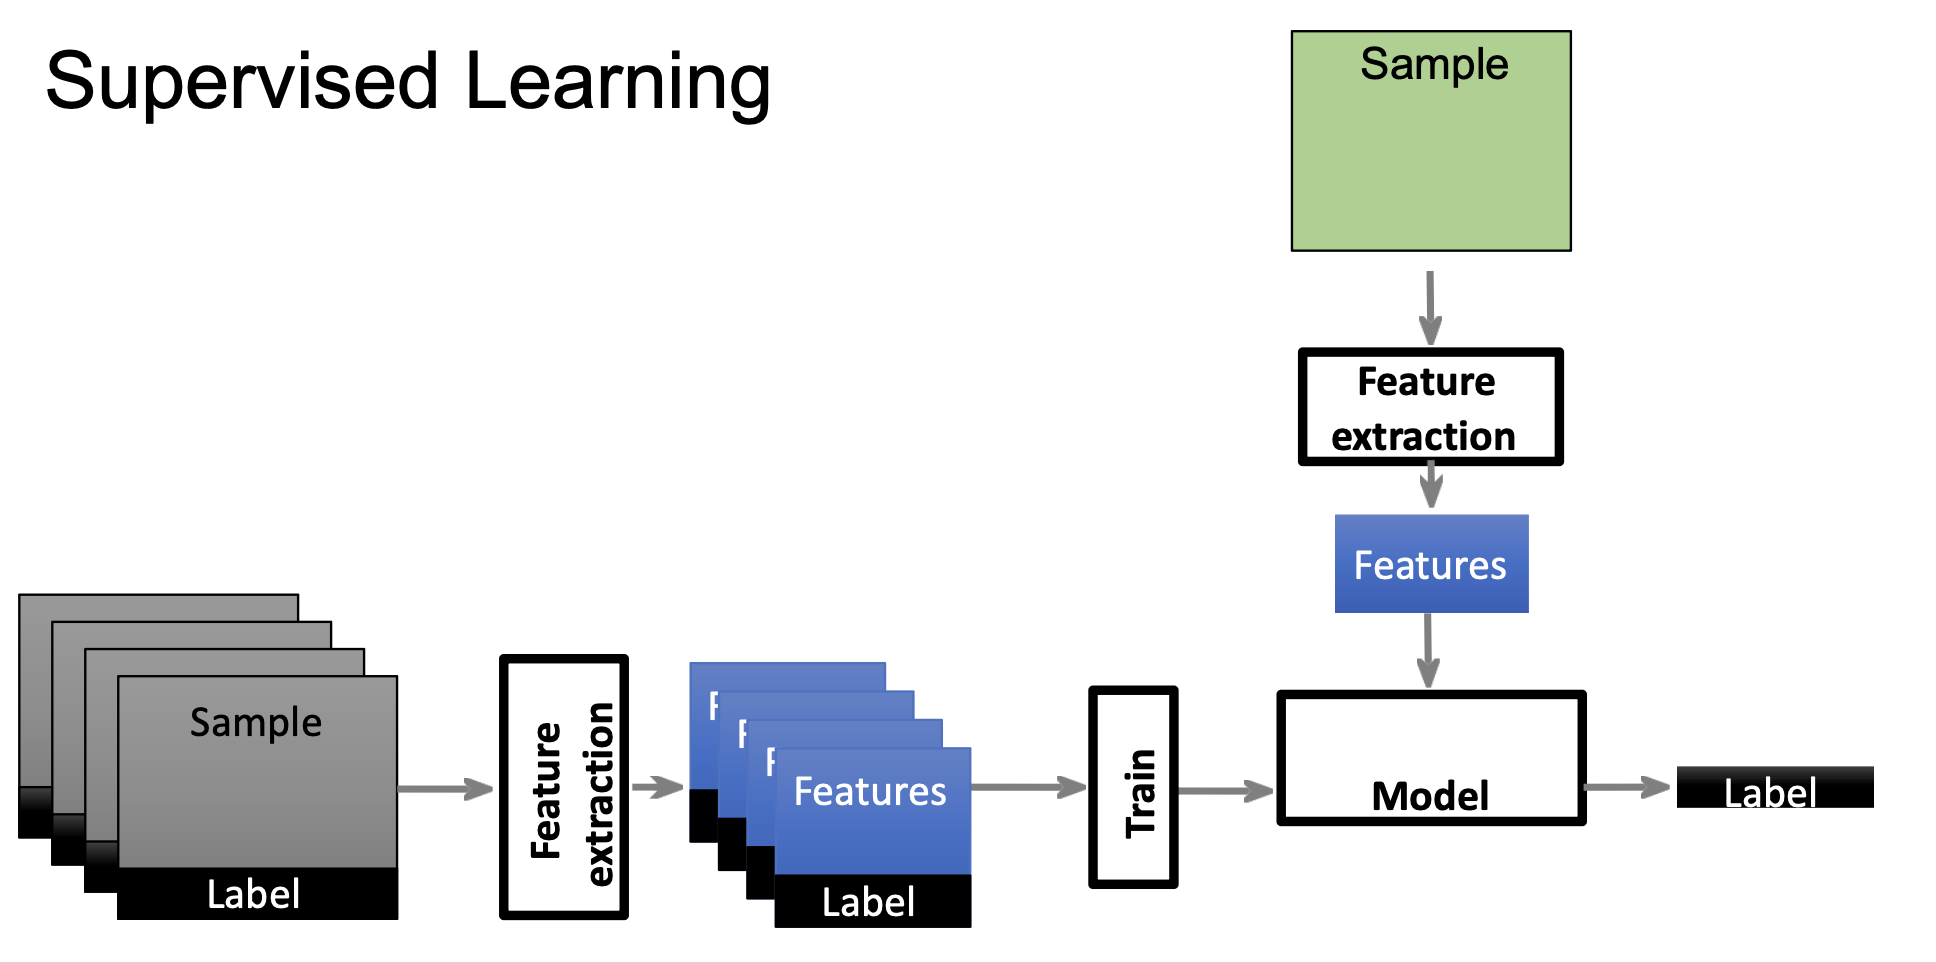
\includegraphics[width=0.8\textwidth]{supervised-learning}
    \label{fig:LABEL}
\end{figure}

\subsection*{Adversary Goals}

\begin{itemize}
	\item Steal information: \textbf{privacy issue}
	\item Steal the model: \textbf{intellectual property}
	\item Alter the output: \textbf{fooling the user}
\end{itemize}

\vspace{0.5cm}

\begin{center}
  {\LARGE \textbf{Model Stealing}} \\
  Protecting intellectual property in ML 
\end{center}
\vspace{0.5cm}

\subsection*{Machine Learning Under Adversarial Conditions}

Up there are the more threatening models, and down is the higher success rates
Opaque-box attacks
\begin{itemize}
	\item Model architecture and parameters unknown
	\item Can only interact \textit{blindly} with the model
\end{itemize}

Grey-box attacks
\begin{itemize}
	\item Model architecture known, parameters unknown
	\item Can only interact with the model, but has information about they type of the model
\end{itemize}

Clear-box attacks
\begin{itemize}
	\item Know architecture and parameters
	\item Can replicate the model and use the model's internal parameters in the attack
\end{itemize}

\subsection*{Machine Learning as a Service}

1. The Cloud, e.g., Amazon ML or Google Prediction API, (pre-)trains a classifier using their own data.

2. Make this classifier available as a service for users to query

3. The user makes a query: "Given their profile (photos, posts, metadata), what pet has this Facebook user?

\vspace{0.5cm}

\section*{Model Stealing}


Confidentiality of the model itself (e.g., intellectual property)

Good ML models require considerable investment:
\begin{itemize}
	\item Collecting data takes time and money
	\item Training infrastructure is expensive (time and \$\$\$)
\end{itemize}

Goal: "steal" the expensive model by observing its outputs with lower cost than obtaining the data and training. 


\subsection*{Stealing a linear model}

Assume adversary knows the model is a linear architecture (\textit{Grey-box model}).

Assume \textcolor{orange}{x} is \textcolor{orange}{two}-dimensional: 
\[
f(x) = w_1 x_1 + w_2 x_2 + b
.\] 

Adversary's goal: steal parameters w, b 

\textbf{How many input-output pairs (x, f(x)) the adversary must observe to steal the model}? 

For \textcolor{orange}{two-dimensional} x only need \textcolor{orange}{3 queries!}

In general, if a linear model users \textit{\textcolor{orange}{d features}}, the adversary needs \textbf{\textcolor{orange}{d+1}} different queries to steal by solving the linear system for w, b

\subsection*{Stealing a non-linear model}

Assume adversary know the model's architecture (\textit{Grey-box model}) \[
f_w(x)
.\] 

Adversary's goal: steal parameters w

\subsection*{Retraining attack}

Observe many queries X = \textit{(x, f(x))}, and fit the model on X like on any other training data! 

Takes many queries. For a neural network with 2K parameters, need 11K queries to get 99.9\% similarity.

More recent work has reduced these numbers. 

\subsection*{More on stealing neural networks}

"Given (oracle) query access to a neural network, learned through stochastic gradient descent, can we extract a \textcolor{orange}{functionality equivalent} model?"

Implication of this attack against neural networks

\textbf{Achievement}: extract a 100,000 parameter neural network on the \textcolor{orange}{MNIST} digit recognition task with $2^{21.5}$ queries in under an hour $\Rightarrow$ implication from cryptographic research for ML

Assumption of the field of secure inference:  \textcolor{orange}{observing the output of a neural network does not reveal the weights}

$\Rightarrow$ This assumption is  \textbf{\underline{false}}, and therefore the field of secure inference will need to develop new techniques to protect the secrecy of trained models

\section*{Preventing model stealing}

First attack = 2016, First defenses $\sim 2017$

\textbf{\textcolor{orange}{Output perturbation}}

Add \textbf{\underline{noise}} to the probabilities output by the model to hinder reconstruction, but not accuracy

\textbf{\textcolor{orange}{Detect suspicious queries}}

Identify deviations from expected on distribution of successive queries from a client 

\begin{center}

	Very recent techniques! We don't yet know how robust they are
\end{center}

\subsection*{Takeaways on model stealing}
\begin{itemize}
	\item Many models are susceptible to stealing
	\item Complex topic, lots of ongoing research
	\item Crucial issue for ML as a service
	\item Very young field, the situation will (probably) improve!
	\item \textbf{\textcolor{red}{Many problems}}, \textbf{\textcolor{green}{some solutions}}
\end{itemize}

\vspace{0.5cm}

\begin{center}
  {\LARGE \textbf{Data Stealing}} \\
  Privacy Challenges in ML
\end{center}
\vspace{0.5cm}

\textbf{Information leaks about data user for training}

\textbf{Testing data (or the result) might be sensitive in ML as a Service}

Questions:
\begin{itemize}
	\item Do trained models leak sensitive data?
	\item Can we train good privacy-preserving models? 
\end{itemize}

\subsection*{Membership Inference}

The attacker tries to understand what data has been used as part of the training. Is a sensitive data point more similar to the "reference" dataset or the "summary statistics"? 

\subsection*{Membership Inference Assumptions}

No knowledge of the model \textbf{parameters} (grey-box attack)

% Quick centered image
\begin{figure}[H]
    \centering
    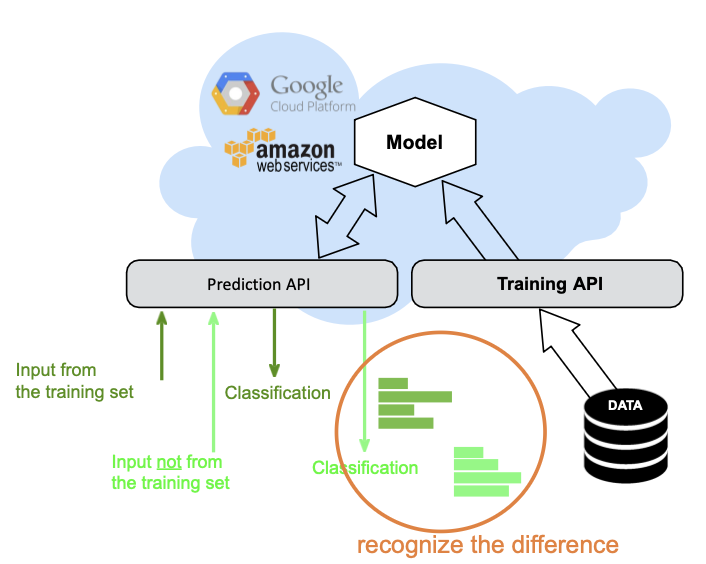
\includegraphics[width=0.8\textwidth]{tm}
    \label{fig:LABEL}
\end{figure}

\begin{tcolorbox}[
  colback=gray!15,     % background color
  colframe=black!50,    % border color
  boxrule=1pt,       % border thickness
  arc=3mm,             % rounded corners
  left=4mm, right=4mm, top=2mm, bottom=2mm % padding
]
\textbf{Attack}

\vspace{0.3cm}
Leverage Public Data for Training, Compare! Without knowing the parameters of the actual model! 
\end{tcolorbox}

Assumptions 2.0: No samples of the training data & no knowledge of the model \textbf{parameters}

\subsection*{Shadow Models}

Try to create \textcolor{orange}{'shadow'} of the actual model to understand how it behave. 

\textbf{Train the attack model} to predict if an input was a member of the training set (in) or a non-member (out) 

% Quick centered image
\begin{figure}[H]
    \centering
    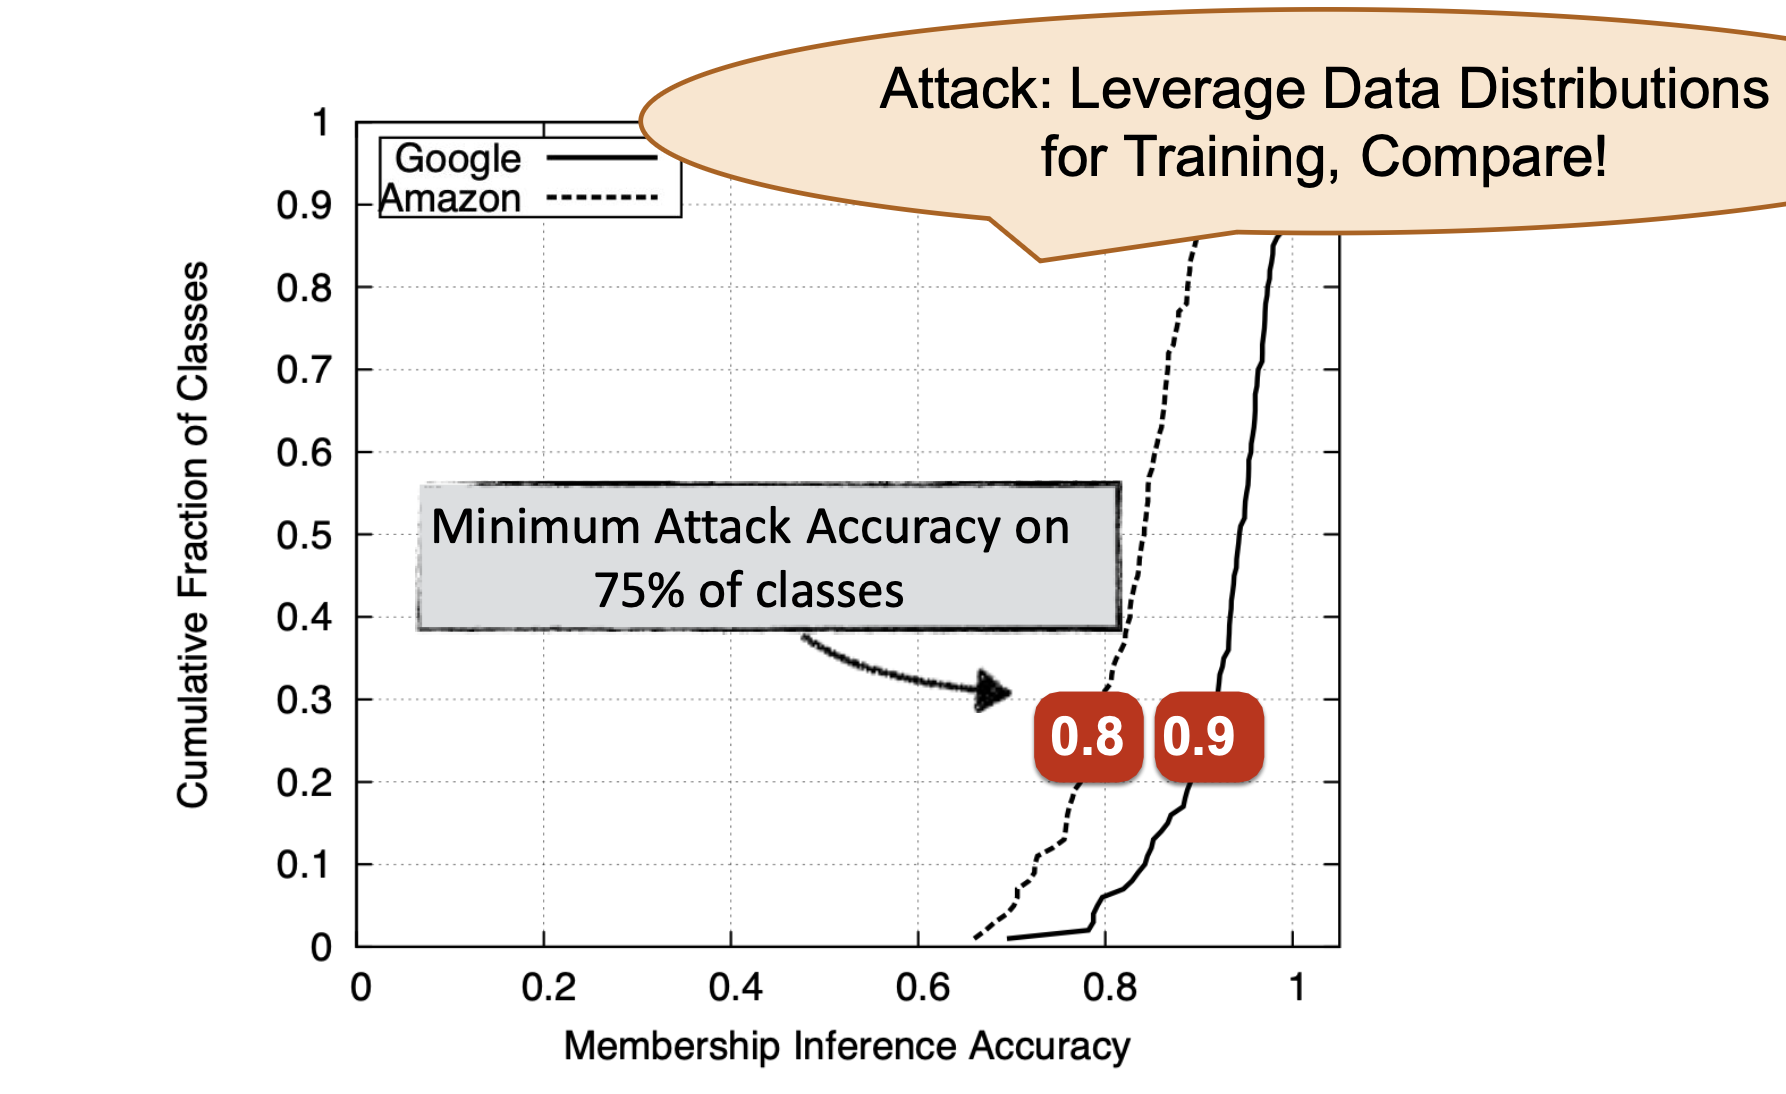
\includegraphics[width=0.6\textwidth]{shadow-model}
    \label{fig:LABEL}
\end{figure}

Assumptions 3.0: No knowledge of the underlying distribution of the \textbf{training data} & no knowledge of the model \textbf{parameters}

\subsection*{Data Synthesis for Shadow Models}

We take random data, use the prediction API to get results and use those to assess distributions. We get very close to the precision of using real data. 

% Quick centered image
\begin{figure}[H]
    \centering
    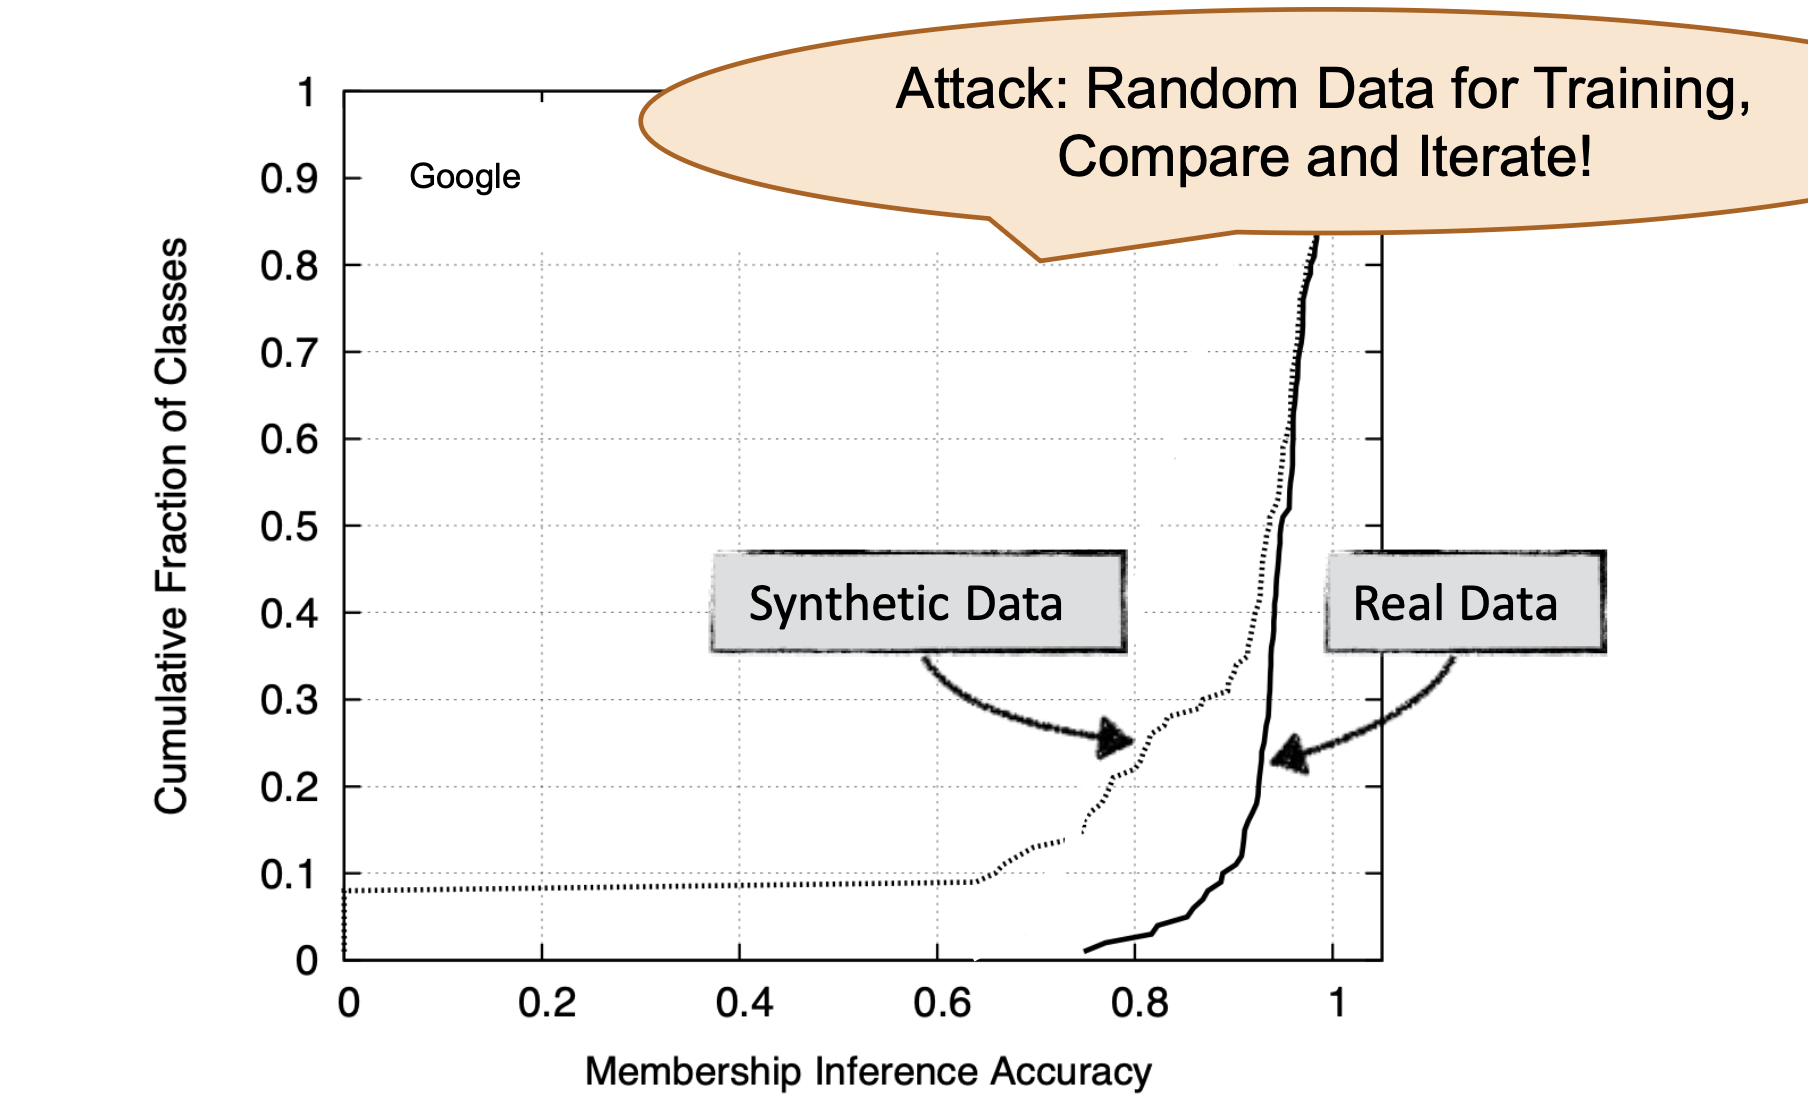
\includegraphics[width=0.6\textwidth]{random-data}
    \label{fig:LABEL}
\end{figure}

\subsection*{Why do these attacks work?}

Because the model is over-fitted on the training data!

\textbf{Overfitting is the common enemy}

\underline{\textbf{Privacy}}: Does the model leak information about data in the training set?

\textbf{\underline{Learning}}: Does the model generalize to data outside the training set?

For once, privacy and utility are \textcolor{orange}{not} in conflict: \textcolor{orange}{overfitting} is the common enemy
\begin{itemize}
	\item Overfitted models leak training data
	\item Overfitted models lack predictive power
\end{itemize}

Need \textcolor{orange}{generalizability} \underline{and} \textcolor{orange}{accuracy}

\subsection*{Takeaways on ML Privacy issues}

\textbf{\textcolor{red}{Many problems}}, \textbf{\textcolor{green}{some solutions}}

\textbf{Very young field, the situation will improve!}

More research needed. 

\vspace{0.5cm}

\begin{center}
  {\LARGE \textbf{Altering the Output}}
\end{center}
\vspace{0.5cm}

\section*{Inputs that will make ML fail}

Inputs to a model that an attacker has designed to cause the model to make a mistake.

Example: a classification model for animals can take a panda photo and adding noise to it (adversarial perturbation), now the models output "Gibbon" instead of "Panda". This happens because of \textbf{overfitting}.

\textcolor{orange}{Independent and Identically Distributed (IID) assumptions no longer hold}

\begin{itemize}
	\item \textit{\textcolor{orange}{Identical}}: inputs are intentionally manipulated to not belong to the training distribution.
	\item \textit{\textcolor{orange}{Independence}}: inputs are no longer draw independently; the attacker may sample from a single input repeatedly. 
\end{itemize}

\subsection*{Machine Learning 101: Quick refresher}

Objective: find model parameters that \textit{\textcolor{orange}{minimize}} empirical loss. How do we "train" those weights? Often, the answer is to use a (simplified) flavor of \textcolor{orange}{gradient descent}.

\subsection*{Adversarial example problem}

\textbf{Goal}: find a perturbation (adversarial noise) that \textit{\textcolor{orange}{maximizes}} loss

\subsection*{How to define similarity?}

The similarity relation is often represented as \textit{adversarial cost constraint}. 

If the goal is to be imperceptible, the common cost is a norm or a perturbation.

\subsection*{Other similarity relations}

Constraint on perturbation norm assumes that similar images are close in, e.g., Euclidean distance. \textcolor{orange}{This is not always true!}

For example, similarity could be defined as small affine transformations (rotations, scaling, ...)  

\subsection*{Transferability Property}

"Adversarial examples have a \textbf{\textcolor{orange}{transferability}} property: 

Samples crafted to mislead a model A are likely to mislead a model B."

\subsection*{Attack Surface}

In the most extreme case, it is possible to construct a single perturbation that will fool a model when added to any image. 

Attackers need minimal resources to attack the system! 

\subsection*{Defending against adversarial examples?}

Defending n general is very head. Can only \textcolor{orange}{defend against a particular threat model} (e.g., perturbations up to epsilon norm), and normally no guarantees. 

Standard ways is \textit{\textcolor{orange}{adversarial training}} (based on \textit{robust optimization)}. It means training on simulated adversarial examples. 

\subsection*{Preventing adversarial examples}

\textcolor{orange}{Certified defenses}

Ensure that no example can exist inside a ball with radius the norm used for the perturbation

\textcolor{orange}{Detect suspicious queries}

Identify deviations from expected on distribution of successive queries from a client

$\Rightarrow$ Unclear whether they are really effective.

\subsection{Takeaways on adversarial examples}

Protecting ML against output alteration (by adversarial examples) is \textbf{\textcolor{orange}{HARD}}

In the adversary controls the inputs in deployed models, they always win! 

Unclear whether there will ever be effective defenses. High-dimensional spaces difficult to characterize

\textit{\textcolor{orange}{Adversarial training}} is the most promising protection technique. 

\begin{tcolorbox}[
  colback=orange!15,     % background color
  colframe=black!50,    % border color
  boxrule=1pt,       % border thickness
  arc=3mm,             % rounded corners
  left=4mm, right=4mm, top=2mm, bottom=2mm % padding
]
If adversarial examples can occur for an ML usage you are considering, be very careful because this can create a severe vulnerability
\end{tcolorbox}

\vspace{0.5cm}

\begin{center}
  {\LARGE \textbf{Biases and Fallacies}}
\end{center}
\vspace{0.5cm}

\section*{Base Rate Fallacy}

We assume equal distribution of cases, if they are not falsely interpret results. 

% Quick centered image
\begin{figure}[H]
    \centering
    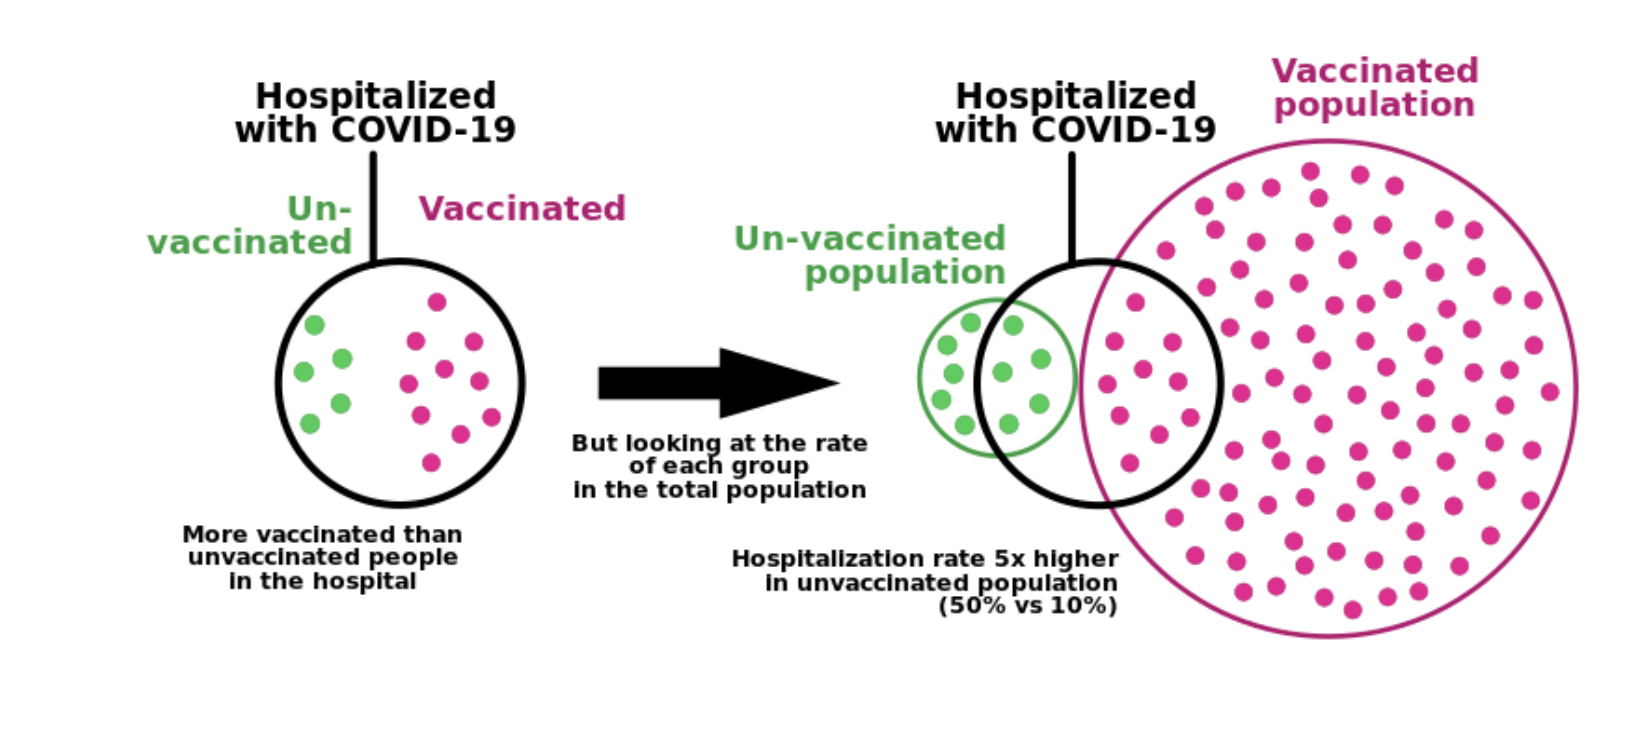
\includegraphics[width=0.8\textwidth]{fallacy}
    \label{fig:LABEL}
\end{figure}

\section*{Prosecutor's fallacy}

\textbf{Quick reminder: AI performance metrics}

\textbf{Example}: Hate speech detection. 

"Only 1 in a million people would match this DNA profile. Therefore, there's only a 1-in-a-million chance the defendant is innocent."

\texttt{P(match $\mid$ innocent)} = 1/1,000,000 $\neq$ \texttt{P(innocent $\mid$ match) = ? }

\subsection*{Distributional Shift}

Distribution of data is not uniform! August 2018 Accuracy on Easy Pilot Parliaments Benchmark in performance on Facial Analysis Task of Gender Classification just works better for lighter males because of data unbalance. 

\subsection*{Controversial ML research}

When the algorithm was presented with two photos where one picture was definitely of a gay man and the other heterosexual, it was able to determine which was which 81\% of the time. With women, the figure was 71\%

What did the algorithm learn?

Faces or stereotypical poses/gestures in the Dating site & Facebook pictures used for training

Would it work in other social networks? Does it work evenly for different races? And for different social groups?

\subsection*{A Bigger Problem: Bias Reinforcement}

Skewed results that overfit because prediction may be biased. 

\textbf{Statistical bias}: difference between an estimator expected value and the true value Very limited! Nothing about errors, nothing about distributional shift

\textbf{Group fairness}: outcome should not differ between demographic groups Predictive parity: same prediction regardless of group (aka, Calibration) Equal false positive (rates)
Equal false negative (rates)
…

\textbf{Individual fairness}: \textcolor{orange}{similar?} individuals should be treated \textcolor{orange}{similarly?}

\subsection*{Takeaways on biases and fallacies}

Deploying machine learning is hard: reality differs far from lab conditions

Base rate matters: it is always hard to get good results on weak signals

Biases come in many flavors, we only say a few examples; it is hard to remove

\end{document}
